\chapter{相关技术基础}

\section{机密计算技术}

\subsection{机密计算概述}
随着云计算、大数据和人工智能技术的蓬勃发展，计算资源正在加速向云端数据中心集中。云计算凭借其高度的资源池化和弹性按需分配机制，为企业和个人用户提供了显著的效率与成本优势。然而这种计算范式的深刻转变也重塑了系统的安全信任边界。在传统的本地计算模型中，用户拥有对物理硬件、操作系统以及上层应用的绝对控制权，而在多租户共享的云环境中，数据所有权与计算环境物理控制权发生了分离，用户不得不将信任单方面赋予云服务提供商及其部署的底层系统软件。在传统的信息安全防御体系中，安全技术主要侧重于保障数据在两种状态下的安全性：一是通过 TLS/SSL 等网络加密协议保护“传输中数据（Data-in-transit）”的机密性与完整性，二是通过全磁盘加密（FDE）和数据库加密技术保护“存储中数据（Data-at-rest）”的安全。然而，当数据被加载到处理器或主存中进行计算与处理，即处于“使用中数据（Data-in-use）”状态时，往往必须以明文形式存在。在传统的特权级架构（如基于 Ring 0/Ring 3 的访问控制）中，操作系统内核和虚拟机监控器（Hypervisor）拥有最高系统权限，能够不受限制地直接读取或修改物理内存。这意味着，一旦底层系统软件存在漏洞被攻击者利用，或者云服务提供商内部存在恶意行为，部署在云端的客户敏感数据（如用户密钥、个人隐私信息、核心业务代码）将面临被轻易窥探或篡改的巨大风险。

为了填补“使用中数据”的安全空白，机密计算（Confidential Computing）技术应运而生。2019年，Linux基金会联合阿里巴巴、AMD、ARM、谷歌、IBM、英特尔、微软等多家行业巨头共同发起成立了机密计算联盟（Confidential Computing Consortium, CCC）。机密计算联盟将机密计算定义为：通过在基于硬件的可信执行环境（Trusted Execution Environment, TEE）中执行计算，来保护使用中数据的机密性与完整性\cite{ccc_whitepaper}。机密计算的核心思想是通过硬件级别的强隔离机制，在不可信的宿主机系统中开辟出一个安全的执行飞地（Enclave）\cite{sabt2015trusted}。在机密计算的底层威胁模型中，传统计算机架构中拥有最高控制权限的系统软件（如操作系统、虚拟机监视器、BIOS及固件等）均被判定为不可信，并被排除在可信计算基（Trusted Computing Base, TCB）之外。这意味着，即使特权系统遭到恶意篡改，或者攻击者对物理内存进行硬件级探测，部署在机密计算环境中的代码和数据依然能免受任何未经授权的读取和修改。在这种架构下，系统的可信基被极大地缩减，通常仅包含底层 CPU 硬件模块及运行在 TEE 内部的应用程序本身，从而在物理与体系结构层面上实现了对上层特权软件的防御。

为了满足不同云计算场景的部署需求，各大主流处理器厂商相继推出了各自的硬件机密计算架构，其保护粒度涵盖了从应用进程级到完整的虚拟机级。作为早期应用级隔离的代表，Intel SGX（Software Guard Extensions）允许开发者将核心敏感代码与数据封装在 TEE 的受保护内存中执行，实现了极小的可信计算基\cite{costan2016intel}。为克服应用级隔离在云生态兼容性与大规模部署上的局限，Intel 随后推出了支持完整虚拟机级别隔离的 TDX（Trust Domain Extensions）技术，利用硬件隔离的信任域实现无修改应用的平移部署\cite{cheng2024intel}。在机密虚拟机（CVMs）领域，AMD 提出的 SEV（Secure Encrypted Virtualization）架构是当前的主流方案之一，它依靠集成在内存控制器中的硬件密码学引擎对虚拟机物理内存进行透明加密，并逐步演进出具备寄存器状态加密（SEV-ES）和内存完整性保护（SEV-SNP）的安全架构\cite{kaplan2016amd}。此外，面向更广泛的计算生态，ARM 推出了 CCA（Confidential Compute Architecture），通过构建机密领域（Realms）为虚拟机或容器级负载提供底层硬件隔离环境\cite{li2022design}。而 IBM 也针对 Power 架构设计了 PEF（Protected Execution Facility）技术，利用安全虚拟机（SVM）与低特权级的安全监控器（Ultravisor）机制，确保云租户数据免受恶意宿主机的窥探与破坏。\cite{hunt2021confidential}

\begin{figure}[htbp]
  %  \vspace{-6em}
  \centering
  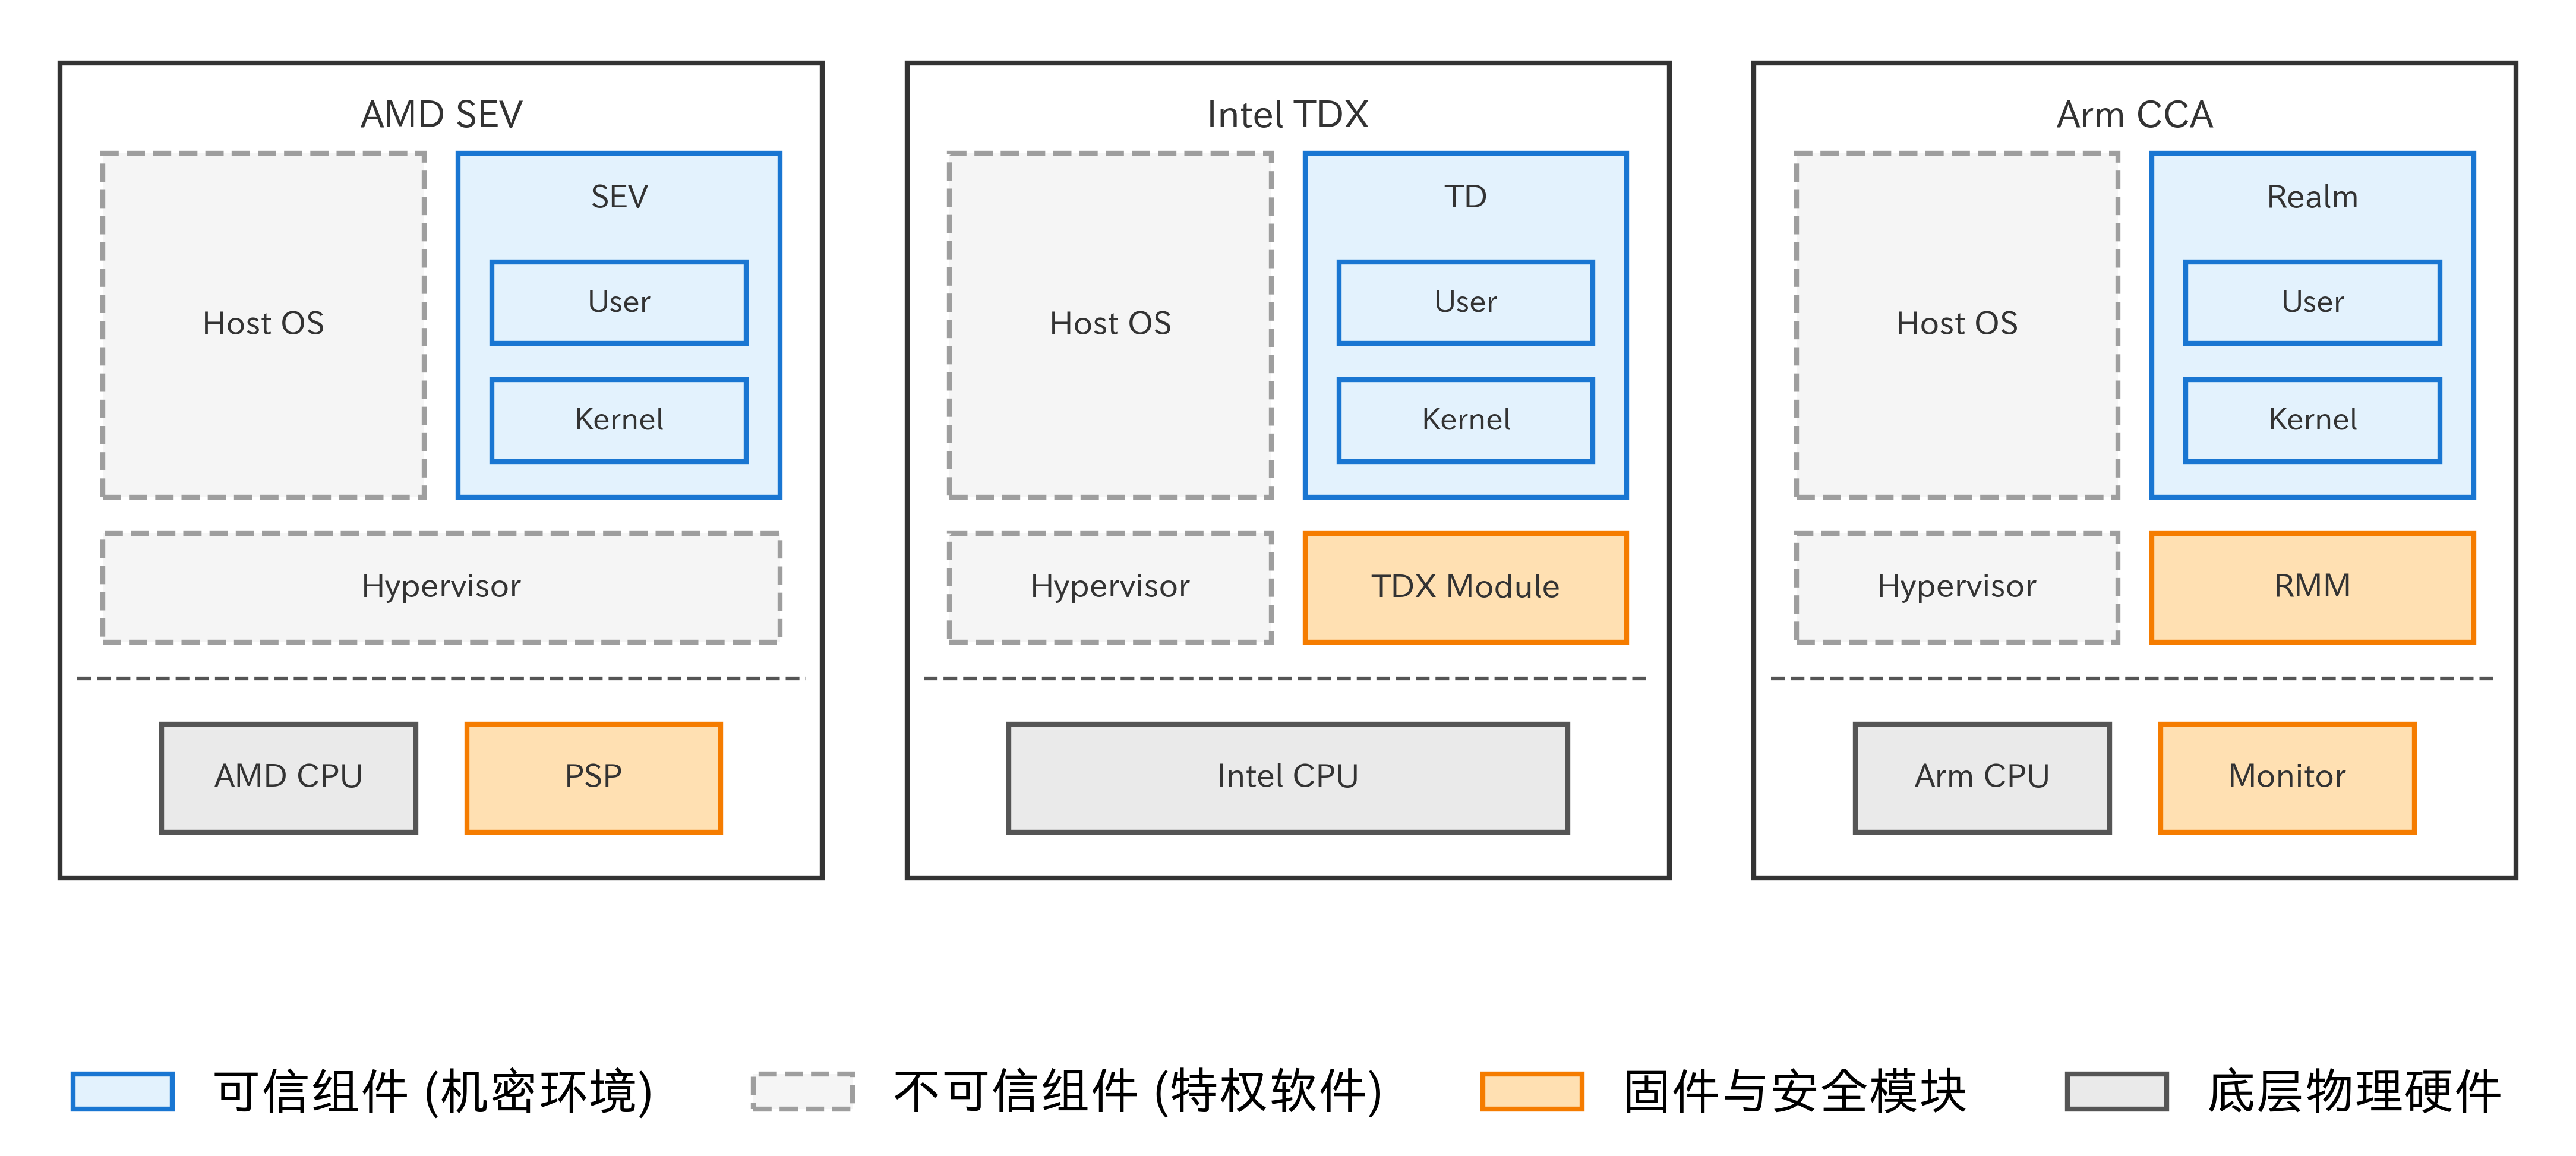
\includegraphics[width = 0.95\textwidth]{pic/tee_arch.png}
  \caption{目前主流的商业可信执行环境架构}
\end{figure}

\subsection{虚拟化与机密虚拟机技术}

虚拟化（Virtualization）是现代云计算平台的核心技术，其目标是在同一套物理硬件之上高效运行多个彼此隔离的操作系统和应用负载。通过在硬件与客户机操作系统之间引入虚拟机监控器（Virtual Machine Monitor, VMM）或 Hypervisor，处理器、内存、存储和网络等物理资源被抽象为逻辑上独立的虚拟资源，使每个虚拟机都能够获得接近独占硬件的运行环境\cite{popek1974formal,barham2003virtualization,kivity2007linux}。这种资源抽象与复用机制显著提升了服务器利用率和云平台弹性部署能力，成为公有云和私有云中的主流计算支撑形式。

从体系结构角度看，虚拟化的基本要求是在不改变客户机操作系统运行语义的前提下，对敏感操作进行有效控制。Popek 与 Goldberg 的经典虚拟化理论指出，一种体系结构若要支持高效虚拟化，其敏感指令应当能够被特权机制捕获，从而由 VMM 接管和模拟\cite{popek1974formal}。然而，早期 x86 平台并不完全满足该条件，业界先后提出了二进制翻译、半虚拟化和硬件辅助虚拟化等多种实现路径。二进制翻译通过动态重写敏感指令绕过体系结构缺陷，半虚拟化通过修改客户机内核并引入 Hypercall 主动与 VMM 协作。而当前主流平台则主要依赖 Intel VT-x 与 AMD-V 等硬件辅助虚拟化扩展，以较低开销实现客户机与宿主机之间的上下文切换和特权控制\cite{adams2006comparison,uhlig2005intel,barham2003virtualization}。

在虚拟化环境中，CPU 虚拟化与内存虚拟化是最关键的两个基础问题。CPU 虚拟化主要负责将客户机中的虚拟 CPU（vCPU）映射到物理 CPU 核心执行，并在中断、异常、I/O 操作和敏感指令发生时切换至 Hypervisor 处理。相比之下，内存虚拟化则涉及复杂的地址空间抽象。如图\ref{fig:virt_address}所示，对于运行中的客户机而言，应用程序首先使用客户机虚拟地址（Guest Virtual Address, GVA）访问内存，随后客户机操作系统通过页表将其转换为客户机物理地址（Guest Physical Address, GPA），但 GPA 并不直接对应真实机器内存，需要由 Hypervisor 再进一步映射到宿主机物理地址（Host Physical Address, HPA）。因此，虚拟化环境中的内存访问通常形成从 GVA 到 GPA，再由 GPA 到 HPA 的两级地址转换链路\cite{bhargava2008accelerating,kivity2007linux}。

\begin{figure}[htbp]
  \centering
  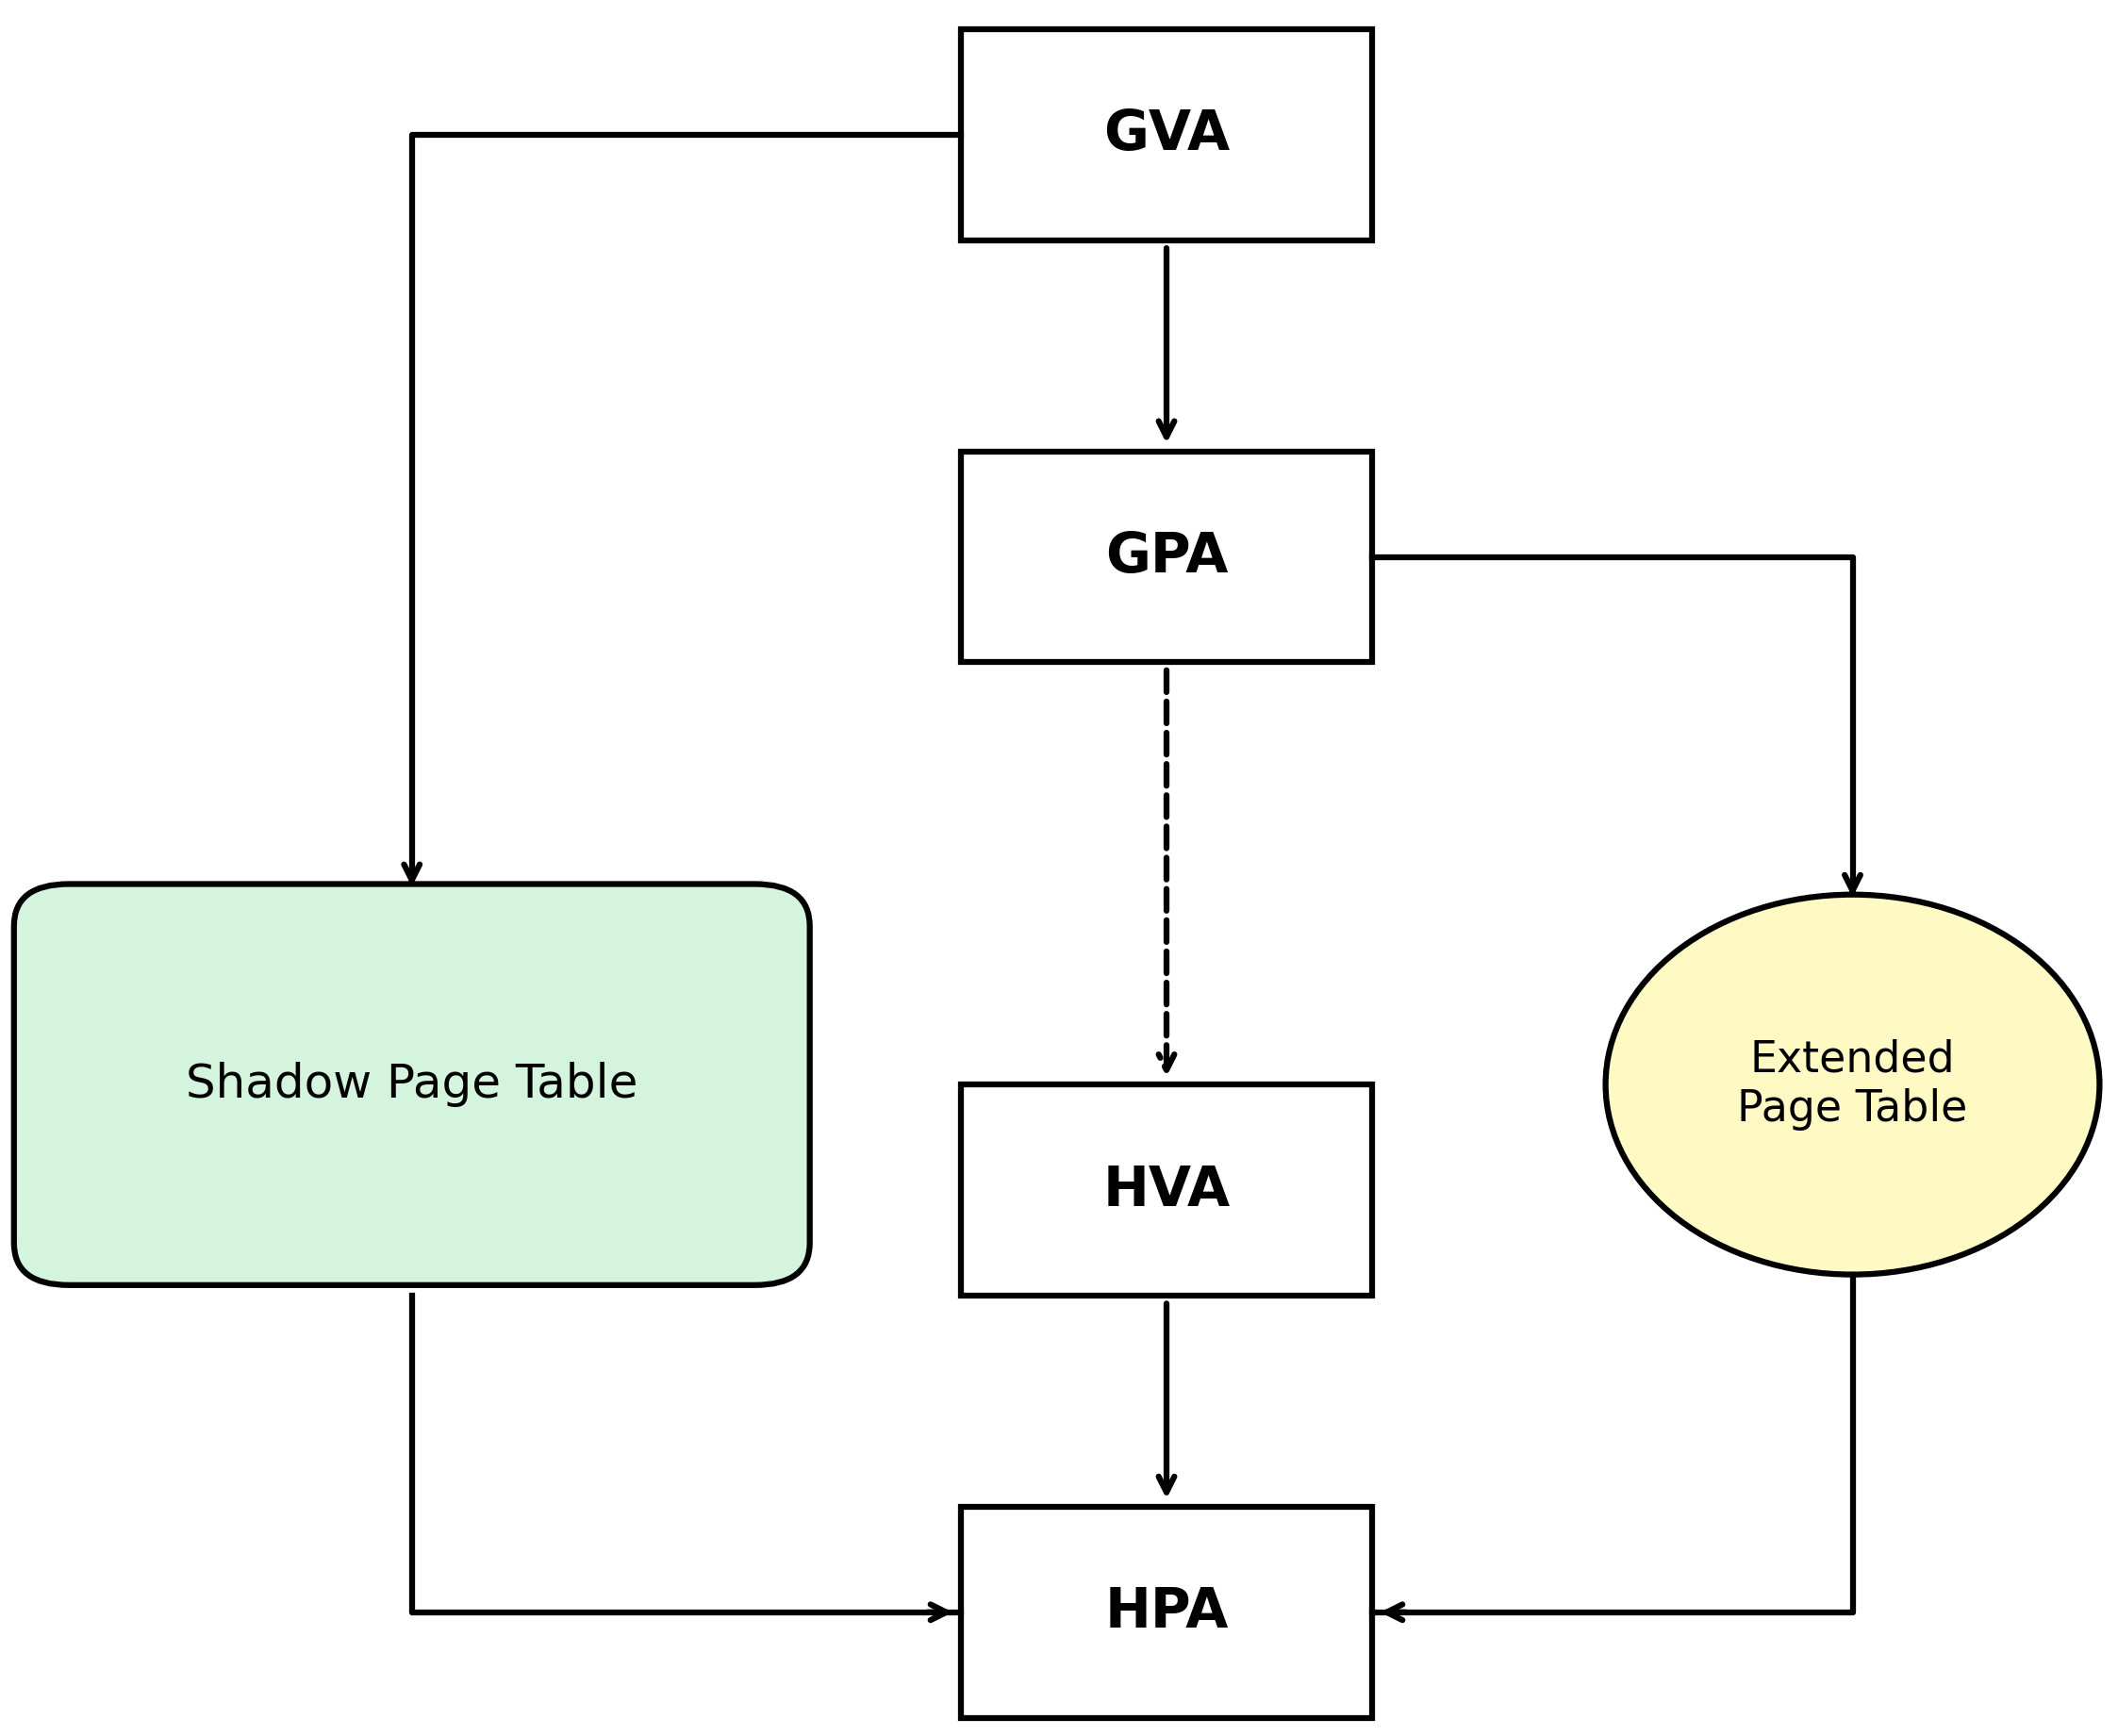
\includegraphics[width = 0.6\textwidth]{pic/virt_address_translation.png}
  \caption{虚拟地址翻译过程}
  \label{fig:virt_address}
\end{figure}

早期虚拟化平台通常采用影子页表（Shadow Page Table）机制来维护最终可供硬件使用的地址映射。具体而言，Hypervisor 将客户机页表与宿主机映射关系合成为一份影子页表，并在客户机页表发生修改时同步更新。该方法能够保证地址转换正确性，但由于客户机页表写入、TLB 刷新和缺页处理需要频繁陷入 Hypervisor，因此会引入较高的运行开销。为解决这一问题，现代处理器普遍提供了硬件支持的两级页表机制，例如 Intel 的 EPT（Extended Page Table）和 AMD 的 NPT（Nested Page Table）。借助这类机制，处理器能够直接在硬件中完成嵌套地址翻译，从而显著减少影子页表维护成本，提高虚拟机访存效率\cite{uhlig2005intel,bhargava2008accelerating}。

除了地址转换之外，Hypervisor 在传统虚拟化中还负责客户机内存的分配、回收、置换、共享和权限控制。例如，Hypervisor 可以决定某一 GPA 是否映射到特定 HPA，可以通过页表项控制客户机页的可读、可写、可执行属性，也可以通过内存超分配、页去重和热迁移等机制提高资源利用率。正因为 Hypervisor 掌握最终的内存映射与调度权，它在传统安全模型中通常被视为完全可信的管理者。然而这一假设同时也带来了显著安全隐患：一旦 Hypervisor、宿主机内核或底层固件遭到攻击，虚拟机的内存内容、执行状态乃至控制流都可能被高权限实体直接观测或篡改\cite{win2014virtual,garfinkel2003virtual}。对于多租户云环境中的敏感业务而言，这种对宿主机平台的强信任依赖显然难以满足“使用中数据”的安全需求。

机密虚拟机（Confidential Virtual Machine, CVM）技术正是在此背景下提出的。其核心思想是在保留虚拟机这一部署形态和云平台兼容性的基础上，借助处理器提供的硬件安全机制，将虚拟机的代码、数据以及关键运行状态封装进一个受保护的执行环境中，使其即使运行在不可信的 Hypervisor 之上，也能够维持较强的机密性与一定程度的完整性保护\cite{ccc_whitepaper,confidentialcomputingconsortium2022}。与 SGX 等应用级可信执行环境相比，机密虚拟机面向的是整机级负载，其优势在于无需对现有应用程序做大规模重构，能够更自然地适配云计算环境中已有的操作系统、中间件和服务框架。

从实现角度看，机密虚拟机通常围绕内存加密、CPU 状态保护、页级完整性校验和远程证明等机制展开。首先，平台会为不同虚拟机分配独立密钥，对其内存数据进行透明加密，以阻止宿主机直接读取明文内容；其次，需要保护虚拟机寄存器状态、异常上下文以及启动测量过程，避免高权限软件在上下文切换或异常处理阶段窃取敏感信息；再次，为防止恶意 Hypervisor 通过重放、重映射或伪造页状态实施攻击，新一代机密虚拟化方案进一步增强了对页归属关系和内存映射一致性的硬件校验能力；远程证明机制允许租户在启动或部署阶段验证当前虚拟机是否运行在符合预期安全策略的平台之上\cite{kaplan2016amd,cheng2024intel,hunt2021confidential}。

目前主流的机密虚拟机架构主要包括 AMD SEV 系列、Intel TDX、Arm CCA 和 IBM PEF。AMD SEV 通过在内存控制路径上实现透明加密来保护虚拟机物理内存，并在后续的 SEV-ES 中扩展到寄存器状态保护，在 SEV-SNP 中进一步引入更强的页状态验证和完整性保护能力\cite{kaplan2016amd}。Intel TDX 以 Trust Domain 为隔离抽象，为每个受保护虚拟机建立独立的硬件安全域，并配套度量与证明机制，以减少 VMM 对客户机内部状态的可见性\cite{cheng2024intel}。Arm CCA 则通过 Realm 机制支持面向虚拟机或容器工作负载的机密执行环境\cite{li2022design}。IBM PEF 则在 OpenPOWER 平台上借助 Ultravisor 构建安全虚拟机管理模型，以降低宿主机管理层对租户计算内容的访问能力\cite{hunt2021confidential}。

机密虚拟机并没有取消传统虚拟化栈对资源管理的作用，Hypervisor 依然承担着虚拟机调度、I/O 转发、设备复用和内存分配等职责；机密的变化主要体现在信任边界的重划分，即 Hypervisor 不再被默认视为完全可信，而是被纳入潜在攻击者模型。机密虚拟化通过硬件手段削弱其对虚拟机内部数据明文的直接访问能力，从而显著提升了云租户对“使用中数据”的保护水平。然而，这类机制主要解决的是高权限软件对内存内容的直接窥探问题，并不能天然消除共享硬件资源所带来的间接泄露风险。例如，多核处理器中的共享缓存、缓存一致性协议、TLB、分支预测器以及内存总线竞争等微架构行为，仍可能在虚拟机与宿主机之间形成可观测的时序差异，为侧信道攻击提供条件\cite{lou2022survey,ge2018survey,chiang2025reloadreload,giner2025coherereload}。

\section{AMD SEV机密计算技术}

\subsection{AMD SEV机密计算概述}

AMD SEV（Secure Encrypted Virtualization）是 AMD 面向云计算虚拟化场景提出的机密计算架构。其设计目标是在尽可能保持现有虚拟机软件栈兼容性的前提下，为虚拟机提供基于硬件的运行时机密性保护\cite{kaplan2016amd,amd64manual}。与传统虚拟化默认信任虚拟机监控器（Hypervisor）的安全模型不同，SEV 将宿主机操作系统、Hypervisor 以及大部分管理软件视为潜在不可信实体，并试图通过硬件内存加密机制削弱它们对客户机明文数据的直接访问能力。对于云租户而言，这意味着虚拟机中的敏感代码和数据在驻留主存时不再以宿主机可直接读取的形式存在，从而在多租户平台上获得了更强的“使用中数据”保护能力。

SEV 的设计思路是以虚拟机为粒度进行透明内存加密。在该架构下，硬件引入了地址空间标识符（Address Space Identifier, ASID）来区分不同的运行实体。底层处理器会为每个受保护的虚拟机分配独立的 ASID，并由内部的安全协处理器生成与之绑定的虚拟机加密密钥（VM Encryption Key, VEK）。虚拟机发出的内存访问请求在写入物理内存（DRAM）前，会由集成在内存控制器中的硬件 AES 引擎自动加密，在重新载入 CPU 缓存前，再由硬件透明解密\cite{kaplan2016amd}。因此，客户机操作系统和应用程序无需感知底层加密过程，也无需修改其正常执行逻辑。这种设计使 SEV 不追求极小化的应用级可信计算基，而是强调对现有虚拟机生态和通用操作系统的兼容性，更适合云原生的整机负载迁移场景。

AMD SEV 的安全能力依赖于多个硬件组件的协同配合，AMD 安全处理器（AMD Secure Processor, AMD-SP）处于可信计算基的核心，负责平台初始化、密钥派生、虚拟机启动测量等安全管理操作；内存加密引擎负责执行硬件级加解密；而 Hypervisor 则被降级为受限的资源调度方，继续承担 vCPU 调度、嵌套页表（NPT）维护和 I/O 模拟等传统职责，但失去了直接读取机密虚拟机内存明文的权限\cite{kaplan2016amd,amd64manual}。

SEV 高度依赖于现有的硬件辅助虚拟化机制（AMD-V 与 NPT），并通过引入加密位（C-bit）扩展了内存寻址逻辑。SEV 虚拟机通过使用客户页面表中的加密位来控制内存页是私有还是共享。如图\ref{fig:cbit}所示，加密位的位置由具体实现决定，通常位于物理地址的高位扩展字段中。共享内存由虚拟机标记为C=0，表示它不需要使用虚拟机的内存加密密钥进行加密。私有内存页仅用于该虚拟机，并标记为C=1。在典型的虚拟机中，大多数页面被标记为私有，只有用于外部通信的选定页面被标记为共享。SEV 通过加密位状态强制约束物理内存的密文存放形式，从而阻止宿主机通过直接读取 SPA 恢复客户机明文\cite{bhargava2008accelerating,kaplan2016amd}。

\begin{figure}[htbp]
  \centering
  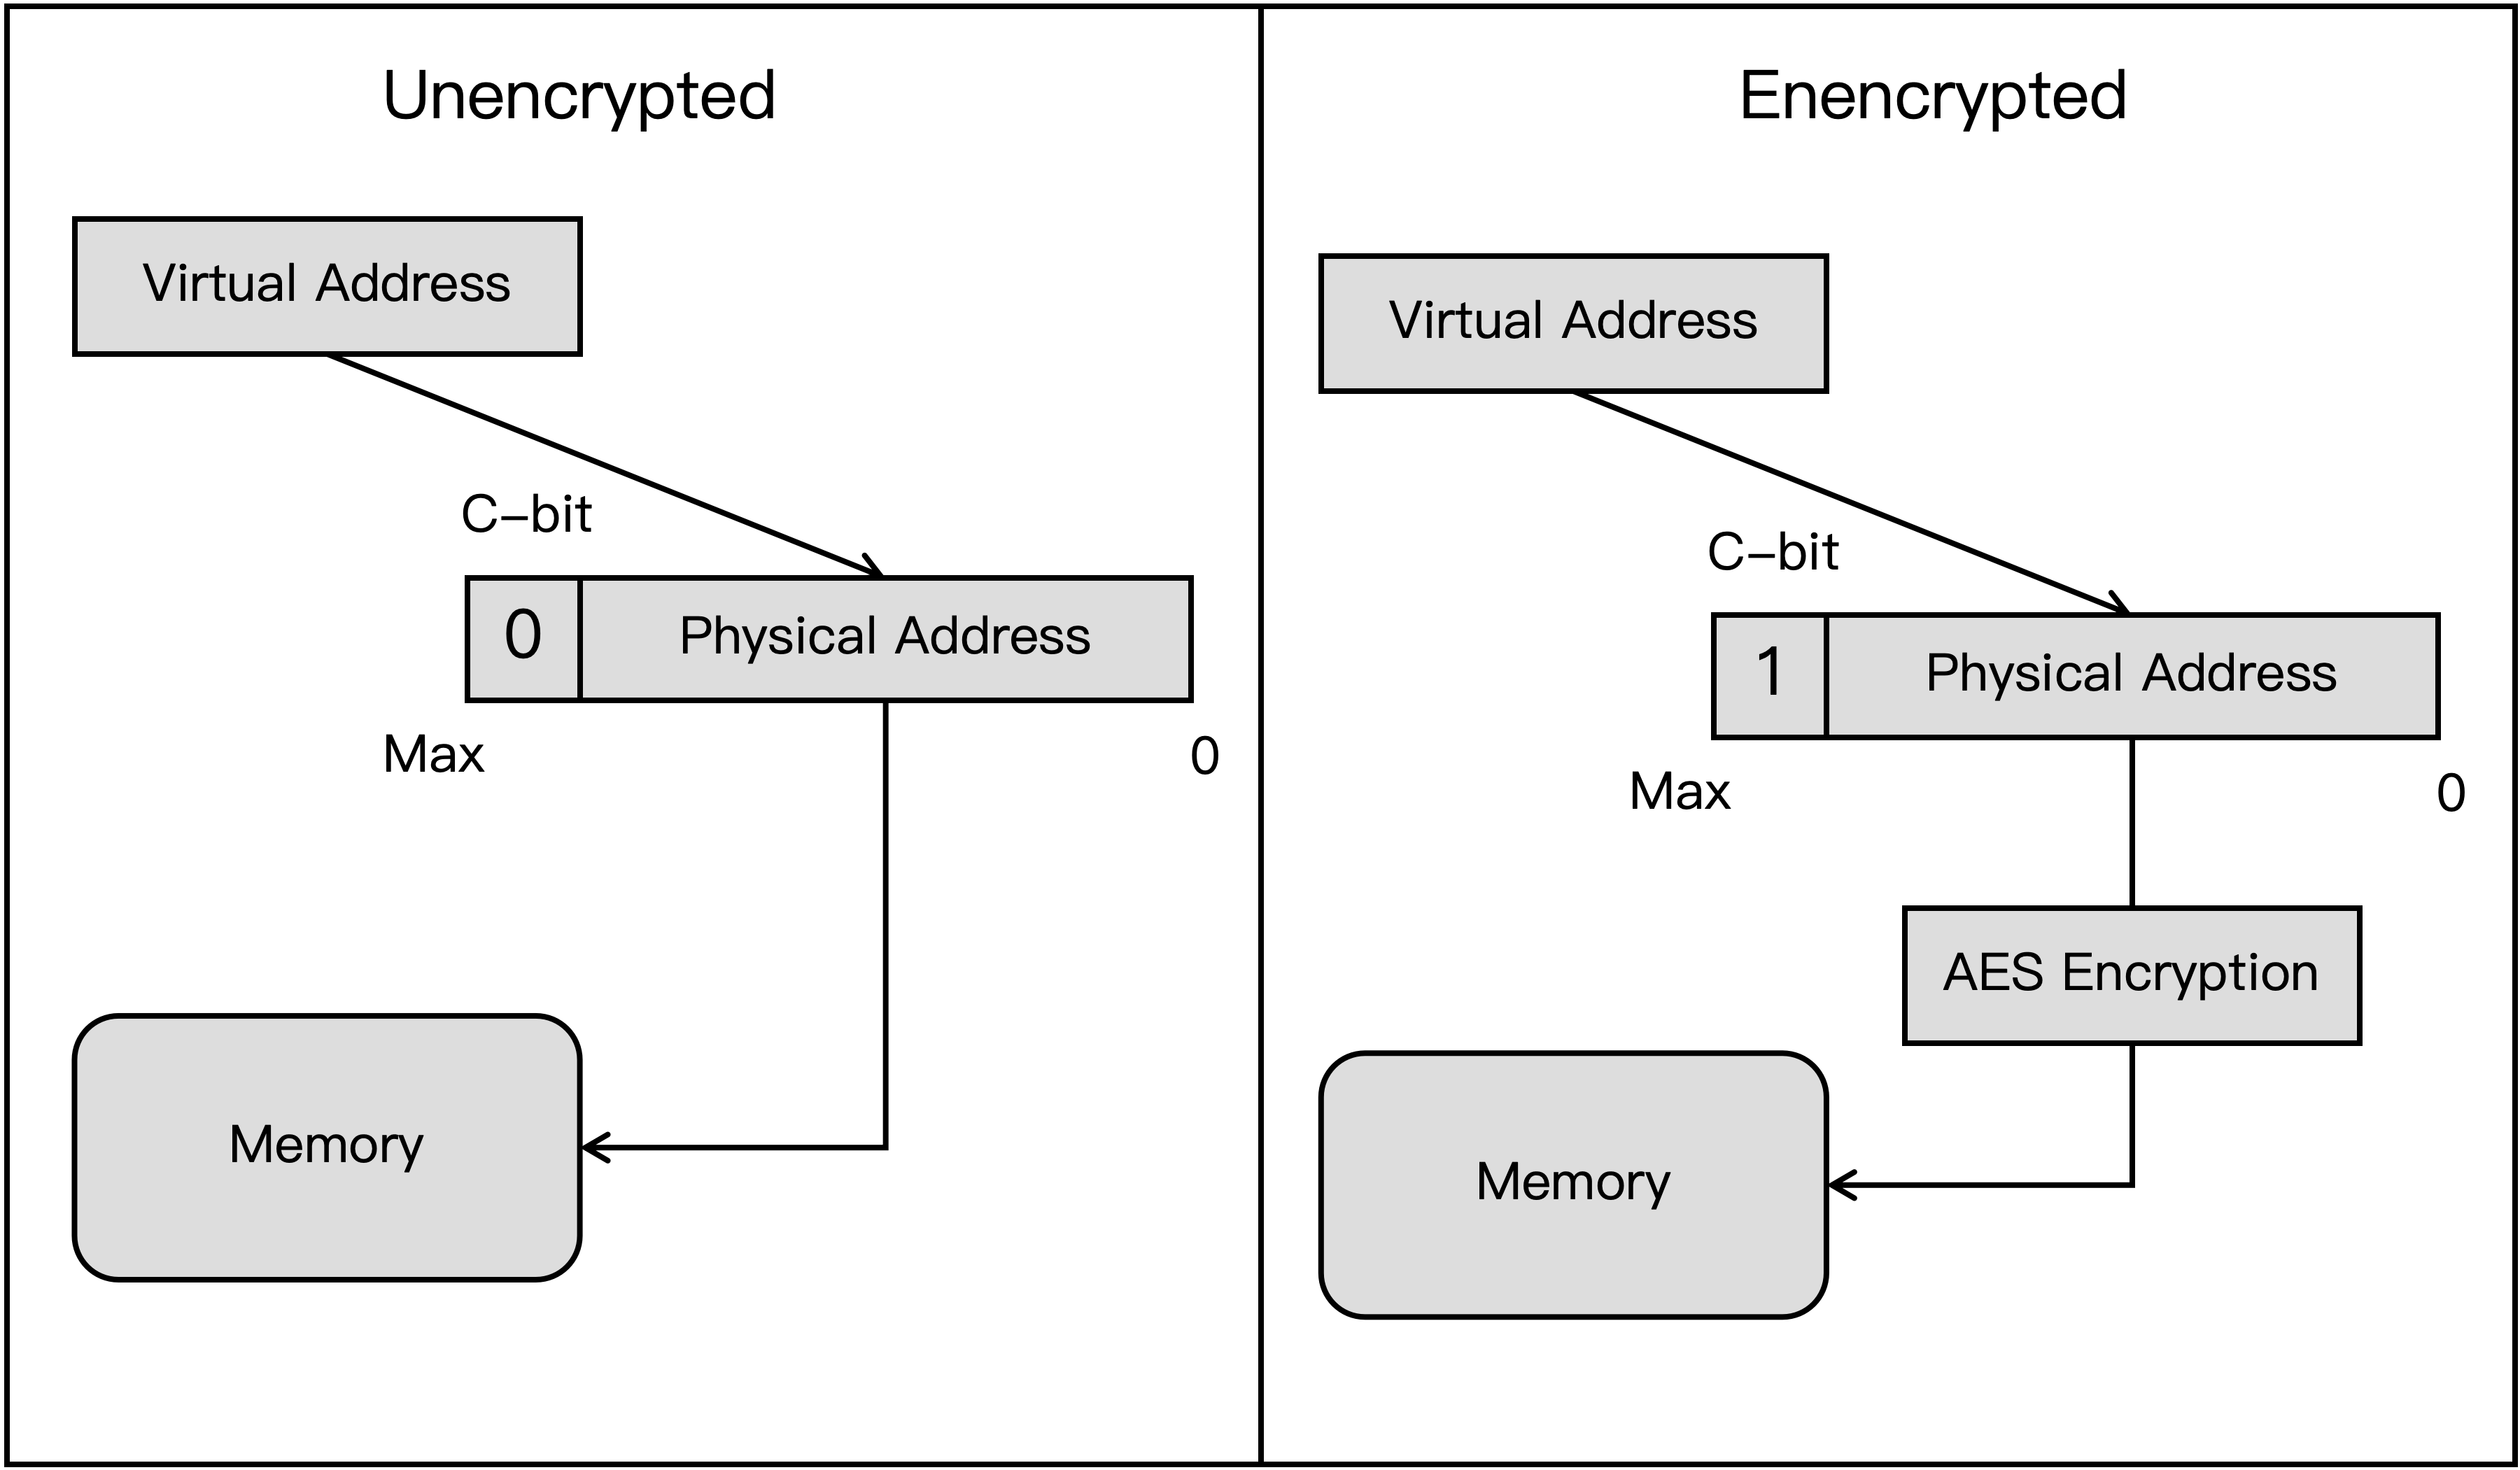
\includegraphics[width = 0.65\textwidth]{pic/Cbit.png}
  \caption{C-bit示意图}
  \label{fig:cbit}
\end{figure}

与传统虚拟机相比，Hypervisor 的安全性决定了虚拟机的安全性。而在 SEV 模型下，信任边界收缩到底层硬件与安全固件\cite{ccc_whitepaper,kaplan2016amd}。然而早期的 SEV 主要解决的是内存机密性问题，并未提供内存完整性保护和寄存器状态保护。恶意的 Hypervisor 仍可能通过篡改页表映射、操纵异常流程等手段实施攻击\cite{morbitzer2018severed}。AMD 继续发展到 SEV-ES 和 SEV-SNP，逐步引入了寄存器状态加密、异常上下文保护以及页状态验证等机制，以增强对恶意 Hypervisor 的防御能力\cite{kaplan2016amd}。但SEV 的内存加密与访问控制机制并不能消除所有底层安全威胁。出于兼容性与性能考虑，CPU 的各级缓存、TLB、分支预测器、缓存一致性协议以及内存总线等微架构资源，仍由宿主机与各个机密虚拟机共享，不可信的 Hypervisor 仍然掌握着系统资源的时空调度权。

\subsection{AMD SEV机密计算技术演进}

AMD SEV 系列的演进过程体现了机密虚拟机安全边界的逐步收紧。初代 SEV 主要面向虚拟机内存机密性，通过按虚拟机粒度的透明内存加密，降低宿主机直接读取客户机明文数据的能力\cite{kaplan2016amd,amd64manual}。然而，后续研究表明，仅依赖内存加密并不足以抵御恶意 Hypervisor；寄存器状态暴露、异常处理路径以及页映射操纵仍可能被利用实施攻击\cite{morbitzer2018severed}。基于此，AMD 又先后提出 SEV-ES 和 SEV-SNP，分别增强执行状态保护与内存完整性保护。

SEV 是该系列的基础版本，其核心机制是为每个虚拟机分配独立的内存加密密钥，并由硬件在内存控制路径上完成透明加解密\cite{kaplan2016amd,amd64manual}。该方案在保持现有虚拟化软件栈兼容性的同时，提高了虚拟机运行时数据的机密性。但在该阶段，VMEXIT 过程中寄存器与部分上下文信息仍可能暴露给 Hypervisor，且后者仍控制嵌套页表与异常注入流程，因此能够通过页重映射、页替换或回放等方式间接影响客户机执行\cite{morbitzer2018severed}。因此，SEV 主要解决的是内存机密性问题，而未能充分覆盖执行状态与内存完整性风险。

SEV-ES 在 SEV 基础上进一步保护客户机执行状态。该机制将大部分 CPU 寄存器状态纳入加密保护范围，从而降低 VMEXIT 后 Hypervisor 对来宾上下文的可见性\cite{amd_sev_es_whitepaper,amd64manual}。同时，SEV-ES 引入 GHCB 作为客户机与 Hypervisor 之间的受控通信接口，使异常处理、I/O 模拟和特权指令模拟等交互仅暴露必要信息\cite{amd_sev_es_whitepaper}。SEV-ES 缩小了 Hypervisor 在退出路径上的观测面，但其增强重点仍集中于执行状态机密性，对页归属验证、内存映射一致性和重放攻击的防护仍然有限。

SEV-SNP 则进一步将保护重点扩展到内存完整性与页状态一致性。该机制在保留内存加密与寄存器状态保护的基础上，引入反向映射表（Reverse Map Table, RMP）记录物理页的归属关系和安全属性，并在地址转换过程中由硬件联合检查页表映射的合法性\cite{amd_sev_snp_whitepaper,amd64manual}。借助 RMP，Hypervisor 对客户机私有页的未授权重映射、属性伪造和非法写入将受到更严格的限制；同时，SEV-SNP 还通过页验证与度量证明机制增强了客户机对初始状态和运行环境的可验证性\cite{amd_sev_snp_whitepaper}。相较于前两代方案，SEV-SNP 在抵御页级篡改、回放和别名映射攻击方面提供了更完整的体系结构支持。

附录表\ref{tab:sev_evolution_threats}给出了 SEV、SEV-ES 与 SEV-SNP 在不同威胁维度下的缓解能力对比。整体上看，SEV 系列的演进路径体现为保护范围由内存机密性逐步扩展到执行状态机密性，并最终延伸到页级完整性与平台可信性。

\section{缓存与缓存一致性}

\subsection{缓存技术概述}

缓存技术的诞生是为了弥补处理器与主存之间的速度差距。随着处理器运算能力持续提升，主存访问延迟逐渐成为制约系统整体性能的重要因素。为降低处理器在访存过程中的等待时间，现代计算机体系结构通常在处理器与主存之间引入多级缓存结构，利用程序访问过程中普遍存在的时间局部性与空间局部性，将近期访问或相邻的数据暂存在速度更高的存储层中，从而减少对主存的直接访问次数，提高平均访存效率\cite{amd64manual}。

如图\ref{fig:cache_arch}所示，现代处理器一般采用层次化缓存设计，包括一级缓存、二级缓存以及最后一级缓存。靠近核心的缓存层容量较小但访问延迟更低，远离核心的缓存层容量较大但访问开销相对更高。该层次结构在容量、成本与性能之间实现了折中，使系统能够在有限硬件资源下获得较优的访存表现\cite{amd64manual}。其中，一级缓存通常进一步划分为指令缓存和数据缓存，以分别服务取指与数据访问；而较高层级缓存则更多承担容量扩展和多核心共享数据缓冲的作用。

\begin{figure}[htbp]
  \centering
  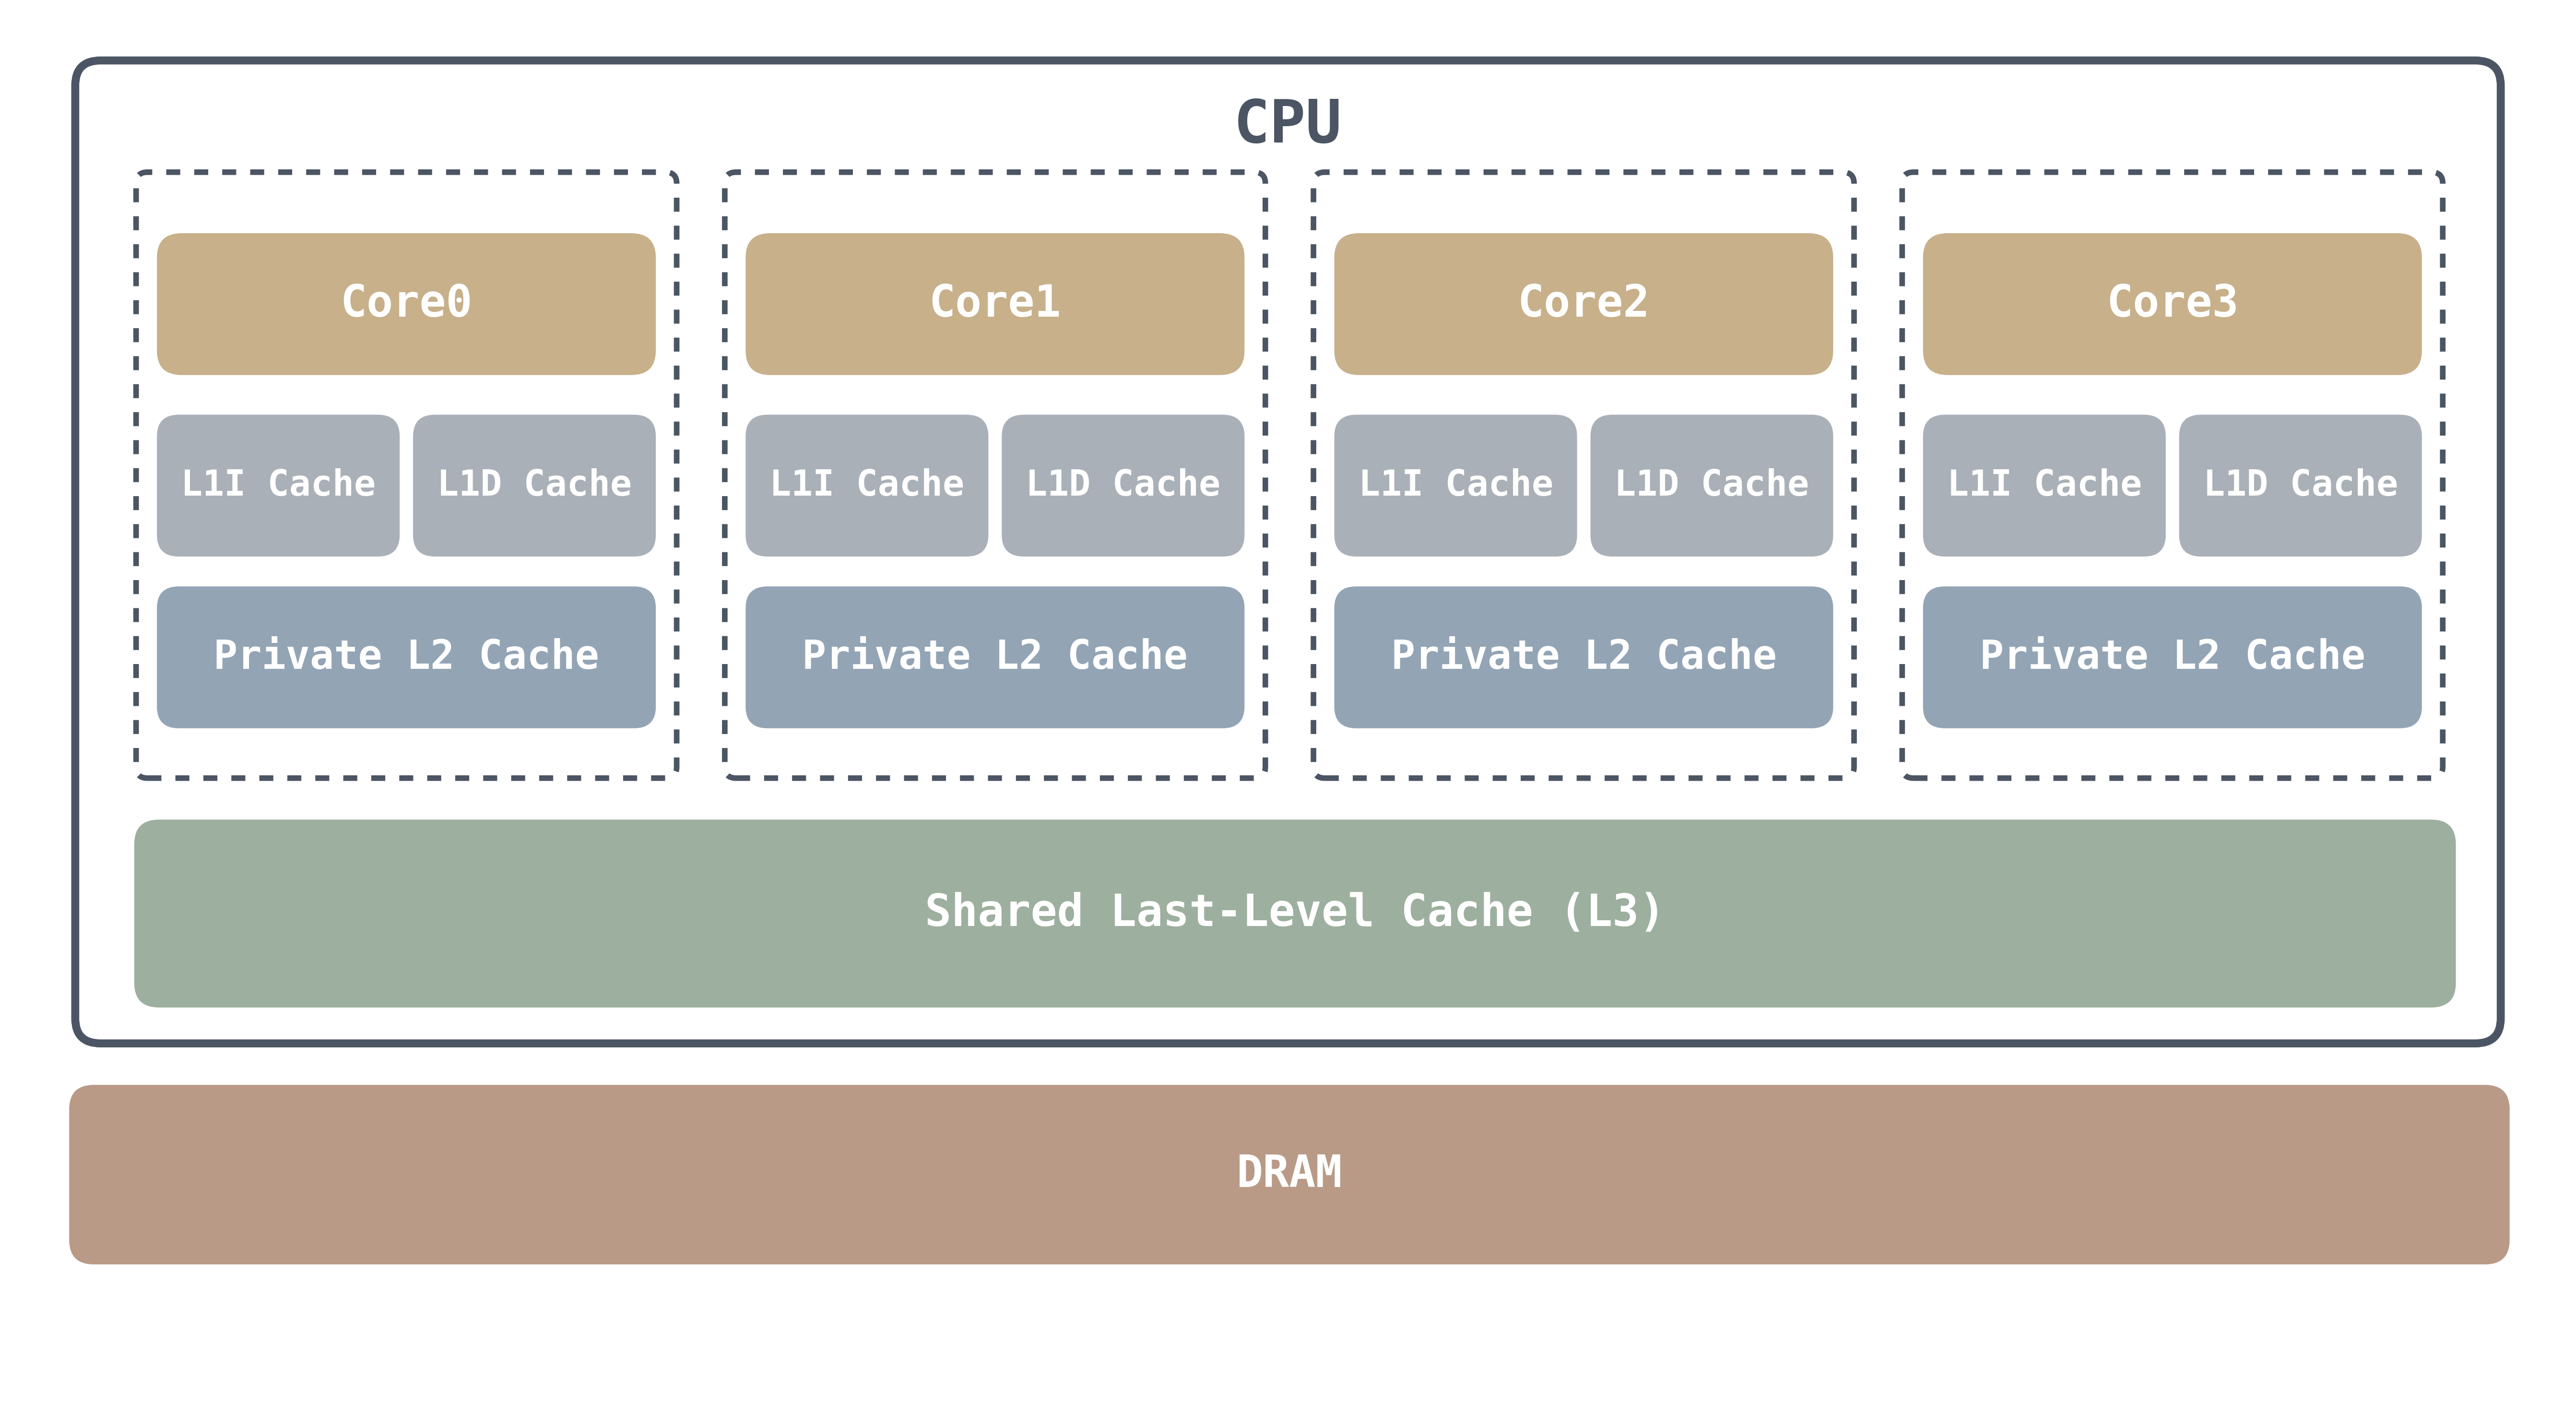
\includegraphics[width = 0.7\textwidth]{pic/cache_arch.png}
  \caption{现代处理器的多级缓存架构示意图}
  \label{fig:cache_arch}
\end{figure}

从组织方式上看，缓存通常以缓存行为基本管理单位，并通过直接映射、组相联或全相联等方式完成地址映射。处理器访问某一内存地址时，需要根据地址中的索引和标记信息判断目标数据是否已存在于对应缓存集合中；若命中，则可直接返回结果，若未命中，则需从下一级缓存或主存装入数据\cite{amd64manual}。因此，缓存命中与缓存未命中之间的访问时延差异，构成了缓存提升系统性能的基本机制。

除映射方式外，缓存系统还涉及替换策略与写策略等关键设计。当前处理器通常采用近似最近最少使用策略进行缓存行替换，并结合写回、写直达、写分配等机制在性能与一致性之间进行平衡。这些设计不仅影响程序执行效率，也决定了缓存状态在不同访问模式下的变化规律。已有研究表明，缓存命中、替换冲突以及共享缓存占用等微架构行为会表现出可观测的时间差异，进而成为性能分析与安全研究的重要基础\cite{osvik2006cache,ge2018survey,lou2022survey}。

在多核处理器环境中，缓存已不再只是单核心的高速缓冲部件，还承担着多核心数据共享与交互中的重要角色。不同核心可能同时缓存同一内存块的副本，私有缓存与共享缓存之间的数据流动也更加复杂。缓存层次结构不仅是提高系统性能的关键机制，也为后续缓存一致性维护以及相关微架构侧信道问题提供了基础。

\subsection{缓存一致性}

在多核处理器中，不同核心可能同时缓存同一物理内存块的副本。为了保证各核心观察到一致的数据视图，处理器需要通过缓存一致性协议协调不同缓存之间的状态变化与数据更新。

常见的缓存一致性协议包括 MESI 和 MOESI。MESI 协议将缓存行划分为修改（Modified）、独占（Exclusive）、共享（Shared）和无效（Invalid）四种状态，用于描述当前缓存副本是否被修改、是否被多个核心共享以及是否仍然有效。当某个核心对共享缓存行执行写操作时，处理器通常需要通过失效其他副本来维持一致性。MOESI 协议则在 MESI 的基础上增加了拥有（Owned）状态，用于表示某个缓存行已经被修改，但其数据可以在不立即回写主存的情况下继续被其他核心共享，从而减少回写开销并提高多核共享场景下的效率\cite{amd64manual}，其状态转移图见附录图\ref{fig:moesi_states}。AMD 处理器在其多核架构中采用了基于 MOESI 的缓存一致性协议，以支持高效的多核心数据共享与交互\cite{amd64manual}。

在机密计算环境中，内存加密机制主要保护的是主存中的数据机密性，而处理器内部的缓存层次结构及一致性维护逻辑通常仍沿用传统多核体系结构。也就是说，机密虚拟机、宿主机以及其他执行实体在运行过程中，仍会通过共享缓存、缓存行迁移、失效广播以及一致性状态转换等微架构行为发生间接交互\cite{lou2022survey,ge2018survey}。这些行为虽然不直接暴露明文数据，但可能在访问延迟、冲突模式和缓存占用上留下可观测差异。对于 AMD SEV-SNP 等机密虚拟化平台而言，机密性的增强并未消除底层共享硬件资源所带来的副作用。

\section{侧信道攻击基础}

\subsection{侧信道攻击概述}
侧信道攻击（Side-Channel Attack）是一类通过分析计算系统在执行过程中产生的物理或微架构特征来推断敏感信息的攻击方法。与传统的基于软件漏洞的攻击不同，侧信道攻击不依赖于系统软件的缺陷，而是利用系统在处理数据时不可避免地泄露出的各种非功能性特征，如时间延迟、电磁辐射、功耗波动、声学信号等\cite{kocher1996timing,kocher1999differential}。这些特征虽然不是设计用来传递信息的，但在特定条件下却能被攻击者捕获和分析，从而揭示出系统内部的秘密状态或敏感数据。

从泄露来源来看，侧信道攻击大致可以分为物理侧信道与微架构侧信道两类。前者主要依赖对设备外部物理现象的观测，例如通过测量功耗、电磁信号或声学噪声恢复算法执行过程中的中间状态；后者则主要针对处理器内部为提升性能而设计的共享硬件结构，如缓存、分支预测器、转换后备缓冲区（TLB）、执行单元以及内存总线等\cite{ge2018survey,lou2022survey}。相比需要接触设备或依赖专用测量仪器的物理侧信道，微架构侧信道往往更适合云计算与虚拟化环境，因为攻击者只需与受害者共享底层硬件资源，便有可能通过时间测量或资源争用观测到与受害者行为相关的细粒度差异。

从一般攻击流程来看，侧信道攻击通常包括触发、观测和推断三个阶段。首先，攻击者需要设法与目标共享某类可观测资源，或诱导目标执行与秘密相关的操作；其次，通过高精度计时、重复采样和统计分析等手段收集侧信道信号；最后，攻击者再将这些观测结果与目标程序的执行路径、访存行为或密码算法中间状态关联起来，从而恢复密钥、访问模式、控制流信息甚至更高层的隐私数据\cite{kocher1996timing,ge2018survey}。由于侧信道信号通常较弱，且容易受到系统噪声、调度扰动和底层硬件机制的影响，攻击的可行性往往不仅取决于理论上的信息泄露，还取决于攻击者是否能够在真实环境中稳定提取和区分这些时间或物理特征。

在云计算和机密计算场景中，侧信道攻击具有更强的现实意义。一方面，云平台中的多租户部署模式使攻击者有机会与受害工作负载共享处理器缓存、内存控制器以及片上互连等底层资源；另一方面，TEE 或机密虚拟机虽然通过内存加密和隔离机制增强了对明文数据的保护，但通常并不会完全隔离处理器内部所有共享微架构状态\cite{lou2022survey,confidentialcomputingconsortium2022}。因此，攻击者即使无法直接读取受保护内存，也可能通过观测共享硬件资源的状态变化来间接推断受害者的敏感行为。这也说明，侧信道攻击突破的并非传统意义上的访问控制边界，而是系统在实现性能优化与资源复用过程中自然暴露出的信息关联。

对于本文关注的 AMD SEV-SNP 机密虚拟机环境而言，侧信道风险主要来自宿主机与机密虚拟机之间仍共享的底层微架构资源。尤其是缓存层次结构、缓存一致性维护逻辑与内存竞争行为，可能在跨加密域访问时形成可观测时延差异。该问题在前文机密虚拟化部分已给出总体背景，这里不再重复展开；下一节将聚焦于可直接用于攻击构造的典型侧信道技术。

\subsection{常见侧信道攻击技术}
从攻击者所利用的信号类型和共享资源来看，常见侧信道攻击技术可以概括为时间侧信道、缓存侧信道、瞬态执行相关侧信道以及功耗、电磁等物理侧信道。这些方法虽然具体实现不同，但本质上都建立在同一个前提之上，即受害者对秘密数据的处理过程会改变底层系统状态，而这种状态变化又会通过时间、资源占用或物理信号的形式被外部观测到。

时间侧信道（Timing Side Channel）是最基础也最早被系统研究的一类方法。其核心思想是利用程序在不同输入或不同密钥条件下执行时间存在差异这一事实，推断内部秘密信息\cite{kocher1996timing}。例如，若密码算法在处理某些中间状态时会触发不同数量的条件分支、循环迭代或访存操作，则整体执行时间可能与密钥比特或数据分布相关。攻击者可以通过大量重复测量与统计分析，从噪声中恢复这种微小的时间偏差。此类思想后来也被扩展到更细粒度的缓存定时分析中，用于远程推断密码实现的访存行为\cite{Bernstein2005CachetimingAO}。时间侧信道实现简单、适用范围广，但其分辨率常受到系统调度、中断和网络抖动等因素影响，因此通常需要大量样本才能稳定提取有效信息。

缓存侧信道（Cache Side Channel）是现代微架构攻击中最典型的一类。由于缓存命中和未命中的访问延迟存在显著差别，攻击者可以通过操控缓存状态并测量自身访问时延，间接判断受害者是否访问了某一缓存集合或缓存行\cite{osvik2006cache,yarom2014flushreload}。围绕 AES 等密码实现的研究已经表明，攻击者可以利用缓存集合冲突、替换行为和重载延迟恢复细粒度的中间状态信息\cite{tromer2010efficient}。典型方法包括 Prime+Probe、Flush+Reload 和 Evict+Reload 等。Prime+Probe 通过先填充目标缓存集合，再在受害者运行后重新访问对应集合，从访问时延中判断缓存是否被受害者替换；Flush+Reload 则依赖共享内存页，先将目标缓存行刷新出缓存，再通过重载延迟判断受害者是否访问过该缓存行。相比一般时间侧信道，缓存侧信道通常具有更高的时间分辨率和空间粒度，因此被广泛用于恢复密码密钥、推断程序控制流以及监控跨虚拟机工作负载行为。

瞬态执行相关侧信道（Transient Execution Side Channel）则利用现代处理器在推测执行、乱序执行和异常回滚过程中的微架构残留状态泄露信息\cite{kocher2020spectre,lipp2018meltdown}。这类攻击的共同特点是：处理器在架构层面最终不会提交非法或错误路径上的执行结果，但在瞬态窗口内已经对缓存、TLB 或其他共享结构产生了可观测影响。攻击者随后可以结合缓存测量等传统侧信道技术，将这些短暂执行留下的微架构痕迹转化为可恢复的秘密数据。Spectre、Meltdown 及其后续变种表明，即使处理器在权限检查和异常处理上满足架构语义，也可能在微架构层面留下足以被利用的信息泄露通道。

除上述依赖时间与共享微架构状态的攻击外，功耗分析、电磁分析和声学分析等物理侧信道同样具有重要研究价值\cite{kocher1999differential,mangard2007power}。功耗分析通过测量芯片在执行不同操作时的瞬时功耗变化，恢复密码算法中间状态或密钥信息；电磁分析则利用处理器、总线或电源模块在工作时产生的电磁辐射推断内部活动，相关研究已经在密码硬件中展示了较强的攻击效果\cite{gandolfi2001electromagnetic}。这类方法往往具有较高的信噪比和较强的恢复能力，尤其在嵌入式设备、智能卡和专用密码模块中应用广泛。但在云计算和虚拟化环境中，由于攻击者通常无法直接接触物理设备，这类攻击的现实门槛相对较高，因此相关研究更多聚焦于能够远程发起的微架构侧信道。

总体而言，不同侧信道攻击技术的差异主要体现在所依赖的泄露媒介、攻击前提条件以及可达到的观测粒度上。时间侧信道依赖总体执行时间差异，前提较弱但精度有限；缓存侧信道依赖共享缓存状态，粒度更细、攻击效果通常更强；瞬态执行攻击则需要处理器存在可利用的推测执行窗口，并往往与缓存测量方法结合使用；物理侧信道虽然在特定场景下恢复能力很强，但通常需要更接近硬件的观测条件。对于机密虚拟机场景而言，最值得关注的正是那些无需突破内存加密边界、仅依赖共享微架构资源即可实施的攻击技术。基于此，本文后续分析将重点放在与缓存、一致性维护以及内存竞争相关的微架构侧信道上。

表\ref{tab:side_channel_techniques_summary} 对常见侧信道技术的主要特征进行了归纳。

\begin{table}[htbp]
  \centering
  \renewcommand{\arraystretch}{1.16}
  \caption{常见侧信道攻击技术总结}
  \label{tab:side_channel_techniques_summary}
  \begin{tabular}{p{1.9cm}p{2.5cm}p{2.6cm}p{2.5cm}p{2.4cm}p{2.2cm}}
    \hline
    技术类型 & 主要观测信号 & 关键前提条件 & 代表方法/工作 & 典型应用场景 & 主要局限 \\
    \hline
    时间侧信道
    & 程序整体或局部执行时延
    & 目标操作时间与秘密相关，且可重复测量
    & Timing Attack\cite{kocher1996timing}，Cache Timing\cite{Bernstein2005CachetimingAO}
    & 远程服务、密码实现分析
    & 信号弱，易受系统噪声和调度扰动影响 \\

    缓存侧信道
    & Cache hit/miss 导致的访问时延差异
    & 共享缓存层次，攻击者可控制或探测缓存状态
    & Prime+Probe\cite{osvik2006cache}，Flush+Reload\cite{yarom2014flushreload}，AES Cache Attack\cite{tromer2010efficient}
    & 跨进程/跨虚拟机监测、密钥恢复
    & 依赖硬件拓扑和共享资源条件，跨平台可迁移性受限 \\

    瞬态执行相关侧信道
    & 推测执行留下的微架构残留（常结合缓存时延）
    & 处理器存在可利用的推测执行窗口或权限检查缺陷
    & Spectre\cite{kocher2020spectre}，Meltdown\cite{lipp2018meltdown}
    & 通用 CPU 与部分 TEE 环境
    & 与具体微架构和补丁状态强相关，复现门槛较高 \\

    物理侧信道
    & 功耗、电磁辐射、声学特征
    & 可接触设备或可部署高精度物理测量手段
    & DPA\cite{kocher1999differential}，EM Analysis\cite{gandolfi2001electromagnetic}，Power Analysis\cite{mangard2007power}
    & 智能卡、嵌入式设备、专用密码硬件
    & 在云环境中通常难以直接获取物理观测通道 \\
    \hline
  \end{tabular}
\end{table}
